\documentclass[fr]{../../../eplsummary}

\usepackage{../../../eplunits}
\usepackage{../../../eplelec}
\usepackage{circuitikz}
\sisetup{detect-all}

\newcommand{\Ueff}{U_\text{eff}}
\newcommand{\Ieff}{I_\text{eff}}
\newcommand{\Umr}{U_\text{moy,r}}
\newcommand{\Imr}{I_\text{moy,r}}

\hypertitle{Convertisseurs électromécaniques}{6}{ELEC}{1310}
{Antoine Paris}
{Bruno Dehez}

\part{Rappels des notions de bases}
Avant tout, rappelons les notations utilisées dans le cours.
\begin{itemize}
	\item Les lettres minuscules $i$ et $u$ décrivent
	la valeur instantanée du courant et de la tension ;
	\item $U_c$, $U_p$ ou $U_\text{max}$ (idem avec $I$)
	donne la valeur de crête (\emph{peak}) de la tension
	(ou de courant) ;
	\item $U$ ou $\Ueff$ (idem avec $I$) donne la
	valeur efficace (ou RMS) de la tension ;
	\item $\Umr$ et $\Imr$ donnent
	la valeur moyenne redressée de la tension et du courant ;
	\item $ff_u$ et $ff_i$ donnent le facteur de forme de
	la tension et du courant. 
\end{itemize}

\section{Définitions}
\begin{mynota}
On note $<g>$ la moyenne d'une fonction quelconque du temps
$g$.
\end{mynota}

\begin{mydef}[Valeur efficace]
\begin{align}
	U = \Ueff & \eqdef \sqrt{<u^2>} & I = \Ieff & \eqdef \sqrt{<i^2>}. 
\end{align}
Dans le cadre de ce cours, et si ce n'est pas précisé, on suppose
toujours que les valeurs données sont des valeurs efficaces.
\end{mydef}

\begin{mydef}[Moyenne redressée]
\begin{align}
	\Umr & \eqdef <|u|> & \Imr & \eqdef <|i|>. 
\end{align}
\end{mydef}

\begin{mydef}[Facteur de forme]
\begin{align}
	ff_u & \eqdef \frac{U}{\Umr} & ff_i & \eqdef \frac{I}{\Imr}. 
\end{align}
\end{mydef}

\subsection{Cas particulier d'une grandeur périodique}
Soit une grandeur $g$. Cette grandeur est \textbf{périodique} si
\[ \exists T \text{ tel que } \forall t \Rightarrow g(t+T)= g(t). \]
On définit alors
\begin{align*}
	f & \eqdef \frac{1}{T} & \omega & \eqdef 2\pi f.
\end{align*}

Dans ce cas particulier, la valeur moyenne devient
\begin{equation}
	<g> = \frac{1}{T} \int_0^T g \dif t
\end{equation}
et la valeur efficace devient
\begin{equation}
	G = \sqrt{<g^2>} = \sqrt{\frac{1}{T} \int_0^T g^2 \dif t}.
\end{equation}

\begin{mydef}[Grandeur alternative]
Une grandeur \textbf{alternative} est une grandeur périodique
de valeur moyenne nulle.
\end{mydef}

\subsection{Cas particulier d'une grandeur sinusoïdale}
Si $g$ est une grandeur sinusoïdale, on peut l'écrire de façon
tout à fait générale
\[ g = G_c \cos(\omega t + \phi_g). \]
En terme de courant et de tension, cela donne
\begin{align}
	u & = U_c \cos(\omega t + \phi_u) & i & = I_c \cos(\omega t + \phi_i).
	\label{eq:sin-form-peak}
\end{align}
Dans ce cas particulier \textbf{uniquement}, on a démonté au cours
de physique 1 que
\begin{align}
	U_c & = \sqrt{2}U & I_c & = \sqrt{2}I.
\end{align}
On peut dont réecrire l'équation \ref{eq:sin-form-peak}
\begin{align}
	u & = \sqrt{2}U \cos(\omega t + \phi_u) & i & = \sqrt{2}I \cos(\omega t + \phi_i).
\end{align}
On préfère en général cette dernière forme car elle utilise les
valeurs efficaces de courant et tension.

\begin{mydef}[Déphasage]
On définit le déphasage $\phi$ entre la tension et le courant
\begin{equation}
	\phi \eqdef \phi_u - \phi_i.
\end{equation}
Si $\phi > 0$, on dit que la tension est en avance sur le courant.
Dans le cas contraire, on dit que la tension est en retard sur le
courant.
\end{mydef}

\section{Phaseurs}
\`{A} chaque grandeur sinusoïdale $g = \sqrt{2}G \cos(\omega t
+ \phi_g)$, on peut associer un \textbf{phaseur}
\begin{equation}
	\bar{G} = Ge^{j\phi_g}.
\end{equation}

\begin{myrem}
Le module du phaseur est égal à la \textbf{valeur efficace} de
la grandeur sinusoïdale.
\end{myrem}

On peut bien sur réecrire ce phaseur en faisant apparaître
une partie réelle et une partie imaginaire et le réprésenter
sur un diagramme phasoriel comme illustré à la figure
\ref{fig:dia-phasoriel}.

\begin{figure}[ht]
	\centering
	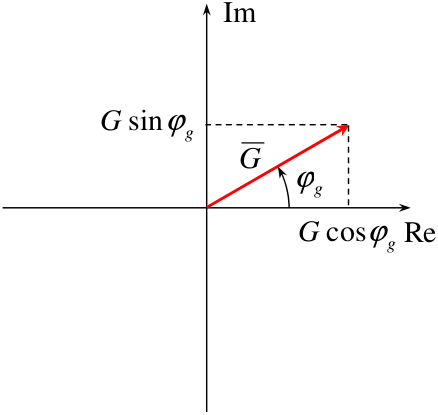
\includegraphics[scale=0.3]{img/dia-phasoriel.png}
\end{figure}

\part{Les transformateurs de puissance}

\part{Les convertisseurs électromécaniques}

\end{document}
